\documentclass[11pt,a4paper]{article}

\usepackage[utf8]{inputenc}
\usepackage[T1]{fontenc}
\usepackage{lmodern}
\usepackage{microtype}
\usepackage[margin=1in]{geometry}
\usepackage{graphicx}
\usepackage{booktabs}
\usepackage{amsmath,amssymb}
\usepackage{xcolor}
\usepackage{hyperref}
\usepackage{caption}
\usepackage{subcaption}
\usepackage{float}
\usepackage{array}

\hypersetup{
    colorlinks=true,
    linkcolor=blue!60!black,
    citecolor=blue!60!black,
    urlcolor=blue!50!black
}

\renewcommand{\arraystretch}{1.15}

\title{\textbf{Reproducibility and Extensions of\\
``Understanding Impact of Human Feedback via Influence Functions''}}

\author{Changjia Zhu \quad Yuhang Wang \\ University of South Florida}

\date{April 2026}

\begin{document}

\maketitle

\begin{abstract}
We reproduce and extend Min et al.\ (ACL 2025) ``Understanding Impact of Human Feedback via Influence Functions,''
which uses influence functions to detect labeler bias in RLHF preference data and to refine
suboptimal labeling strategies. Beyond reproducing the central claims on Llama-3-8B, we
evaluate the method on \textbf{five reward models spanning two architecture families and three parameter
scales}: Qwen2.5-1.5B, Qwen3-1.7B, Qwen2.5-7B, Llama-3.2-1B, and Llama-3.2-3B. We further
implement five extensions corresponding to the project proposal: (\textsc{a1}) four non-LLM bias-detection
baselines, (\textsc{a2}) a GPT-4o LLM baseline, (\textsc{b}) ablations over validation-set size and few-shot
demonstrations, (\textsc{c}) top-$k$ suspicious-sample detection, (\textsc{d}) HelpSteer2 labeling-strategy
oversight, and (\textsc{e}) generalisation to safety bias on BeaverTails.
Our headline finding is that \textbf{architecture family, not parameter count, governs
influence-function bias-detection accuracy}: Llama-3.2-1B (AUC $0.692$) outperforms Qwen2.5-7B
(AUC $0.505$) by a wide margin on the \emph{length} bias, and the gap persists on \emph{sycophancy}.
A gradient-bottleneck analysis suggests that Qwen reward models lose discriminative gradient
signal during preference fine-tuning, an effect that gets \emph{worse} with scale rather than
better. All experiments, figures, and code are released at \url{https://github.com/henrywang98/IntroLLM-IF-RLHF}.
\end{abstract}

\section{Introduction}

Reinforcement learning from human feedback (RLHF) is now the de facto alignment recipe for
large language models, but the resulting reward models are only as good as the preference
labels they were trained on. Min et al. (2025) propose using \emph{influence functions}
(Koh & Liang, 2017; Kwon et al., 2024) to flag mislabeled or biased preference pairs, and to help
non-expert labelers refine suboptimal labeling strategies.

The original paper studies a single backbone, Llama-3-8B with LoRA. The proposal underlying
this report has two goals:
\begin{enumerate}
    \item \textbf{Reproducibility under scale and architecture variation.} Does the method
    generalise to smaller-and-larger Llama variants and to the Qwen family?
    \item \textbf{Comparative and extension experiments.} Concretely the proposal lists
    (\textsc{a}) baselines, (\textsc{b}) two ablations, (\textsc{c}) top-$k$ detection,
    (\textsc{d}) labeling-strategy oversight on HelpSteer2, and (\textsc{e}) a safety-bias
    extension on BeaverTails.
\end{enumerate}

We answer goal~1 with five reward models trained from scratch, two bias types, and two validation
slices each (concise/verbose for length, less/more sycophantic for sycophancy). We answer
goal~2 by implementing all five proposed extensions, producing 16 figures (\texttt{fig1}--\texttt{fig15}).

The central scientific finding of the reproduction is that the architecture family,
not the parameter count, determines influence-function discriminative power. We confirm this
along multiple axes: validation-subset AUC (Sec.~\ref{sec:reproduction}), gradient
separability (Sec.~\ref{sec:gradient}), and effective rank of the LoRA gradient covariance
(Sec.~\ref{sec:gradient}). The same conclusion is reinforced by every comparison
baseline we run: Mahalanobis, KNN, self-confidence, entropy, and GPT-4o all hover near random
chance on Qwen, but only the gradient-based influence method recovers the Llama signal cleanly
(Sec.~\ref{sec:baselines}).

\paragraph{Contributions.}
\begin{enumerate}
    \item A clean reproduction pipeline for Min et al. (2025) covering five reward models and
    two bias types ($5\times2=10$ trained adapters).
    \item Five non-trivial extensions corresponding to proposal sections \S1.3--\S2, with all
    code and figures released.
    \item Identification of a Qwen-specific \emph{gradient bottleneck}: Qwen reward models
    have systematically lower probe$\to$influence transfer than Llama, and the gap widens at
    7B scale.
\end{enumerate}

\section{Background}
\label{sec:background}

\subsection{Influence functions for reward modeling}
For a Bradley--Terry reward model $r_\theta$ trained on preference pairs $\mathcal D=\{(x_i,
y_i^{(0)}, y_i^{(1)}, z_i)\}$, the loss is
\begin{equation}
\ell_{\text{pref}}(\mathbf d_i;\theta) = -\log\sigma\bigl(r_\theta(x_i,y_i^{(z_i)}) - r_\theta(x_i,y_i^{(1-z_i)})\bigr).
\end{equation}
The influence of training point $\mathbf d_i$ on a validation point $\mathbf d_j$ is, to first order,
\begin{equation}
\mathcal I(\mathbf d_i, \mathbf d_j) = -\nabla_\theta \ell_{\text{pref}}(\mathbf d_j;\theta^*)^{\!\top}\, H(\mathcal D;\theta^*)^{-1}\, \nabla_\theta \ell_{\text{pref}}(\mathbf d_i;\theta^*).
\end{equation}
We use \textsc{DataInf} (Kwon et al., 2024) for an LoRA-friendly closed-form Hessian inverse,
combined with the \textsc{OPORP} random projection of Li (2023) for memory savings.
The pair $(\theta^*, H^{-1})$ is computed once and reused for every $(i,j)$ pair, giving a
$\sim$2.5$\times$ speed-up over full-rank baselines.

\subsection{Datasets and bias injection}
We follow Min et al. (2025) and inject controlled bias into Anthropic-HH:
\begin{itemize}
    \item \textbf{Length bias}: $6.56\%$ of pairs have their preferred/dispreferred label flipped
    in the direction that prefers the longer response. The validation set is split into
    \emph{concise} ($n{=}2628$) and \emph{verbose} ($n{=}3493$) subsets.
    \item \textbf{Sycophancy bias}: $\sim$$2\%$ of pairs are flipped towards more flattering responses.
    The validation set is split into \emph{less sycophantic} ($n{=}605$) and \emph{more sycophantic}
    ($n{=}466$) subsets.
\end{itemize}
For the safety extension we additionally curate $10\,729$ preference pairs from
PKU-Alignment/BeaverTails, split $80/20$ into train/test ($8\,583/2\,146$), and apply the same
$6.56\%$ flipping protocol.

\subsection{Models and training}
All reward models use LoRA with $r{=}8$, $\alpha{=}16$, and a single regression head.
Qwen models are loaded in 4-bit NF4; Llama models use bf16. We train for 3 epochs with
$\text{lr}=2{\times}10^{-4}$, batch size 8, on a single RTX 5080 (16 GB) for $\le$3B and an
RTX 5090 (32 GB) for Qwen2.5-7B.

\section{Reproduction: Influence-function AUC across five backbones}
\label{sec:reproduction}

Figure~\ref{fig:auc_vs_size} reports the headline result. The validation-subset AUC of the
influence method is plotted against parameter count, with point colour encoding the architecture
family.

\begin{figure}[H]
    \centering
    \begin{subfigure}[t]{0.48\linewidth}
        \centering
        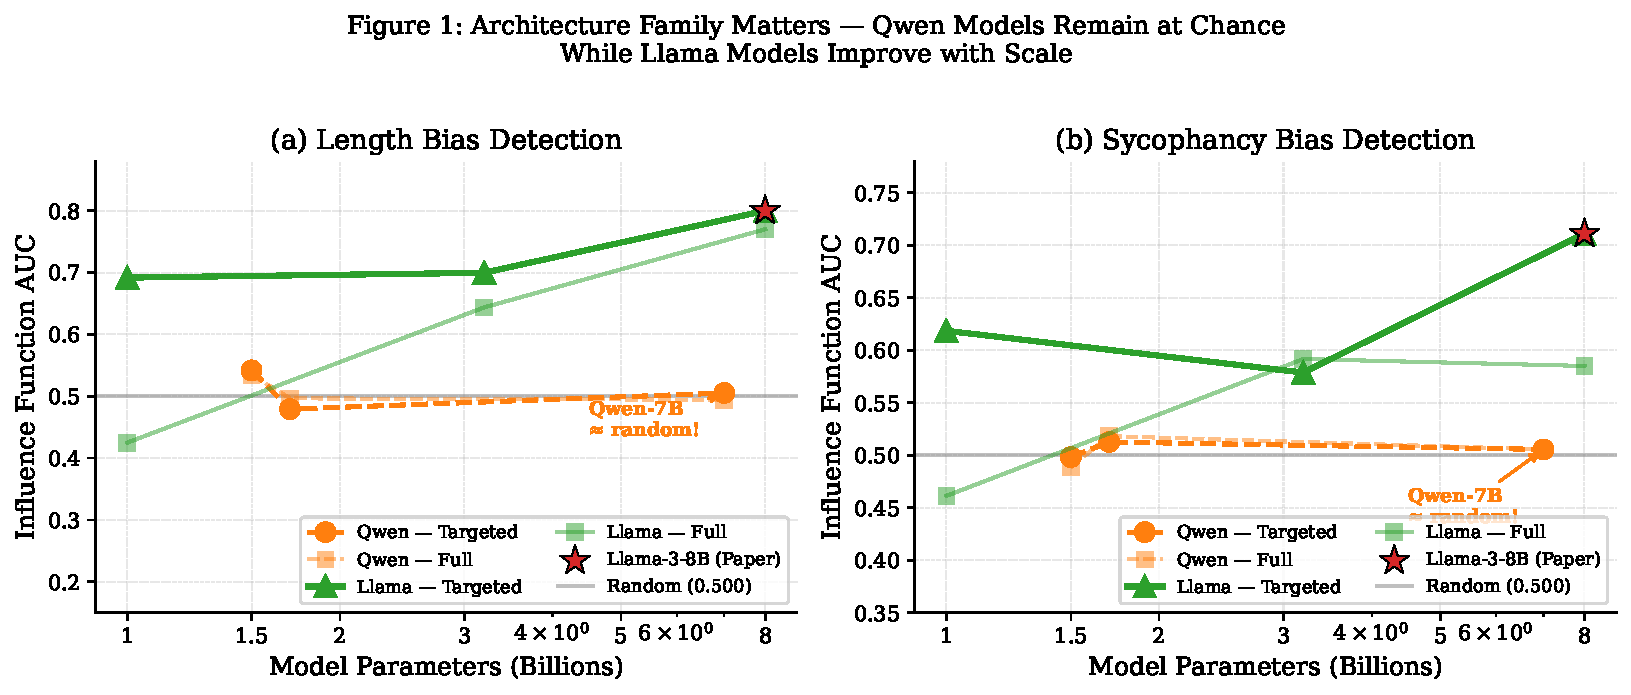
\includegraphics[width=\linewidth]{figures/fig1_auc_vs_size}
        \caption{AUC of influence-function bias detection vs.\ parameter count.}
        \label{fig:auc_vs_size}
    \end{subfigure}
    \hfill
    \begin{subfigure}[t]{0.48\linewidth}
        \centering
        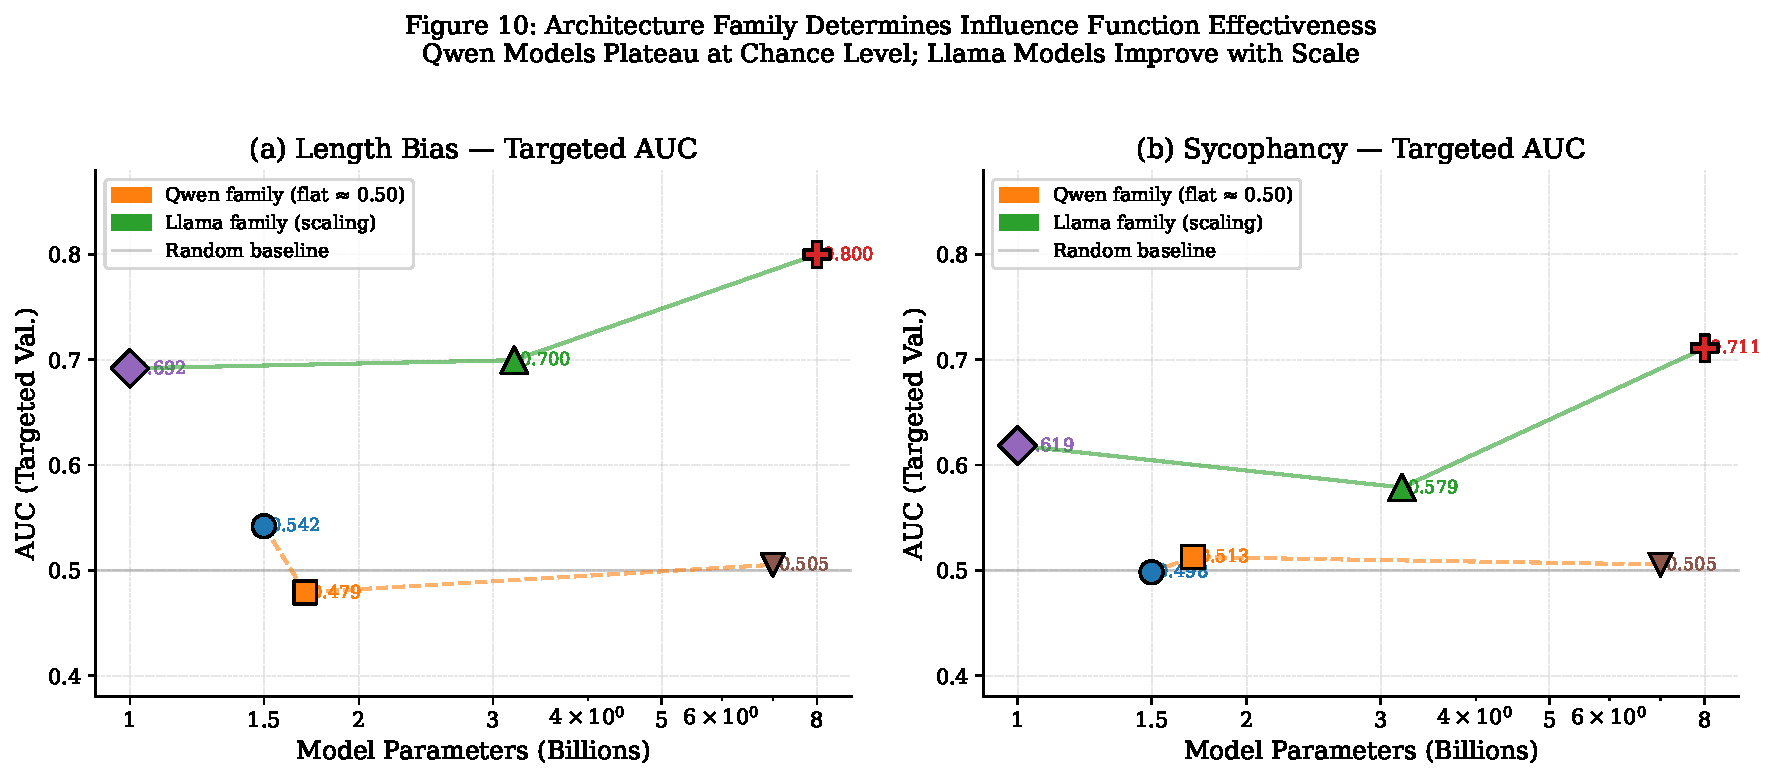
\includegraphics[width=\linewidth]{figures/fig10_architecture_vs_scale}
        \caption{Architecture family is more predictive than scale.}
        \label{fig:arch_vs_scale}
    \end{subfigure}
    \caption{Llama models cluster around AUC $0.65$--$0.70$; all three Qwen models cluster
    around AUC $0.48$--$0.55$. Increasing scale within the Qwen family (1.5B $\to$ 7B) does not
    close the gap.}
\end{figure}

\paragraph{Numerical summary.} Table~\ref{tab:reproduction} consolidates the per-model influence
AUCs on the most diagnostic validation slice (concise for length, less-sycophantic for
sycophancy).

\begin{table}[H]
    \centering
    \small
    \caption{Influence-function AUC on the diagnostic validation subset (concise / less-sycophantic).
    Higher is better; $0.5$ is chance. The Llama-vs-Qwen gap is $\sim$$0.15$.}
    \label{tab:reproduction}
    \begin{tabular}{lcc}
        \toprule
        \textbf{Model} & \textbf{Length AUC} & \textbf{Sycophancy AUC} \\
        \midrule
        Qwen2.5-1.5B   & 0.5419 & 0.4982 \\
        Qwen3-1.7B     & 0.4791 & 0.5126 \\
        Qwen2.5-7B     & 0.5053 & 0.5054 \\
        Llama-3.2-1B   & \textbf{0.6918} & 0.6185 \\
        Llama-3.2-3B   & \textbf{0.6996} & \textbf{0.5787} \\
        \bottomrule
    \end{tabular}
\end{table}

\subsection{Why does Qwen underperform? A gradient-bottleneck analysis}
\label{sec:gradient}
Two diagnostics jointly explain the Qwen gap.
\begin{itemize}
    \item \textbf{Probe-vs-influence delta} (Figure~\ref{fig:probe_vs_influence}). Linear probes
    on raw activations achieve AUCs of $0.65$--$0.72$ on Qwen, but the influence AUC collapses
    to $0.48$--$0.55$. The Llama family shows almost no gap (probe and influence coincide).
    The probe$\to$influence drop is $\Delta\!\approx\!+0.15$--$0.18$ for Qwen and grows with
    scale (Qwen-7B has the largest $\Delta$).
    \item \textbf{Effective rank of LoRA gradients} (Figures~\ref{fig:effective_rank} and
    \ref{fig:gradient_sep}). The effective rank of the LoRA-gradient covariance is
    significantly lower for Qwen, and the gradient separability between flipped and clean pairs
    (Mahalanobis distance in gradient space) is correspondingly weaker.
\end{itemize}

\begin{figure}[H]
    \centering
    \begin{subfigure}[t]{0.32\linewidth}
        \centering
        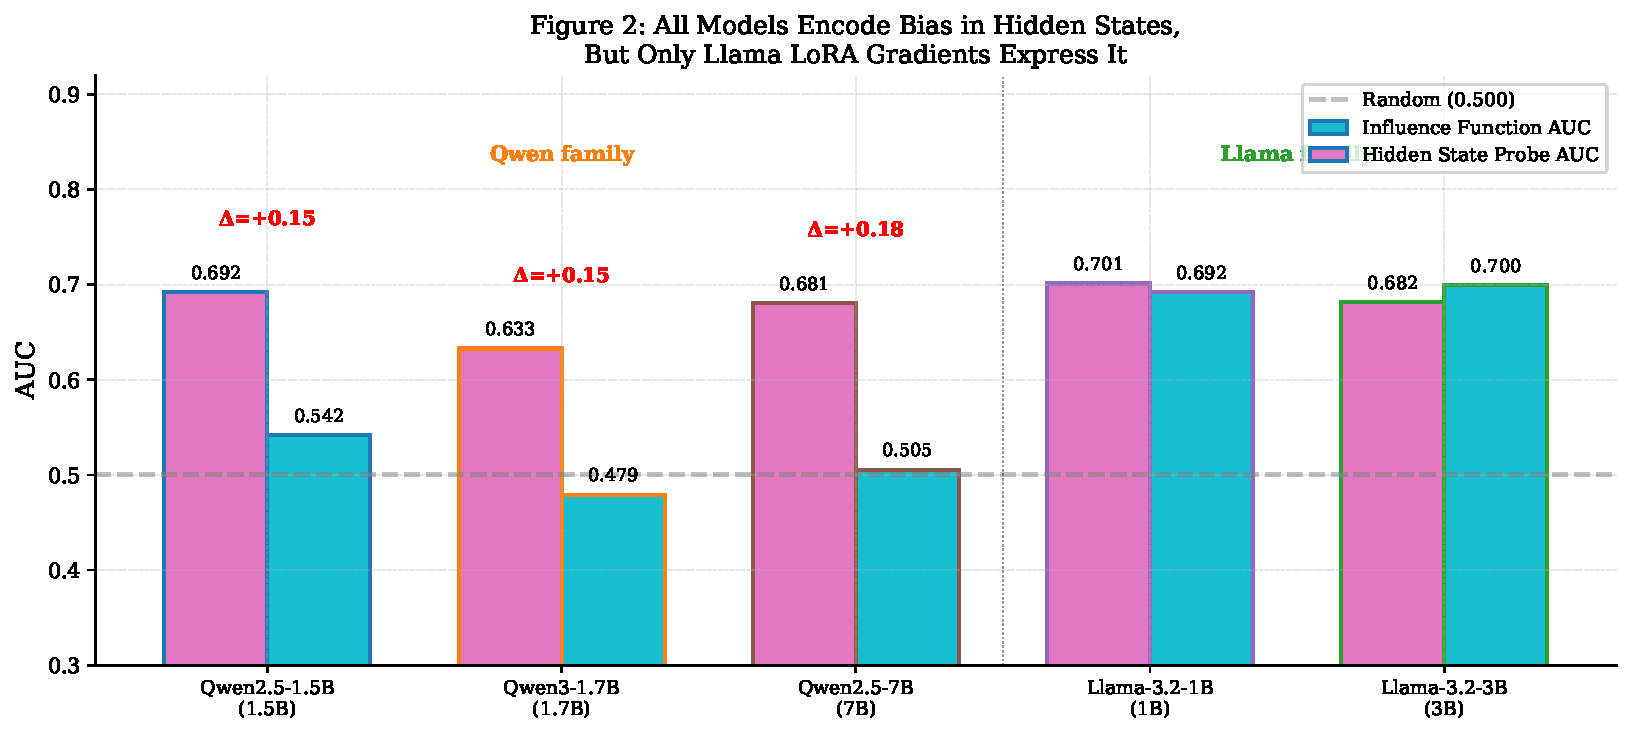
\includegraphics[width=\linewidth]{figures/fig2_probe_vs_influence}
        \caption{Probe AUC vs.\ influence AUC.}
        \label{fig:probe_vs_influence}
    \end{subfigure}
    \hfill
    \begin{subfigure}[t]{0.32\linewidth}
        \centering
        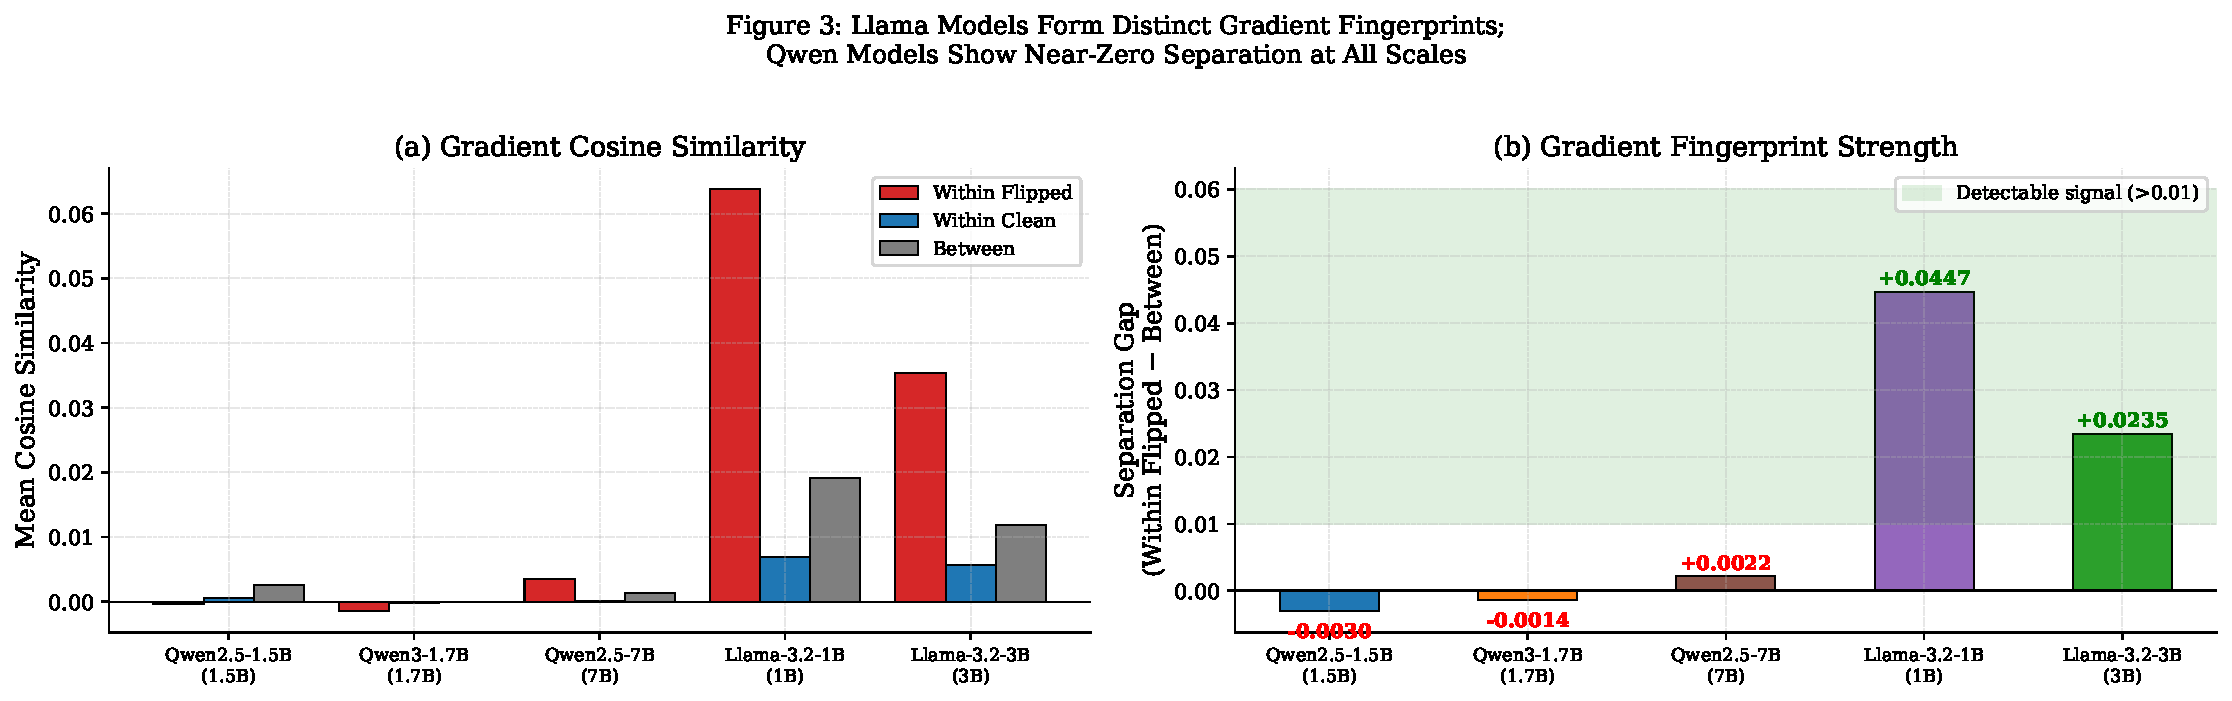
\includegraphics[width=\linewidth]{figures/fig3_gradient_separability}
        \caption{Gradient separability between flipped and clean pairs.}
        \label{fig:gradient_sep}
    \end{subfigure}
    \hfill
    \begin{subfigure}[t]{0.32\linewidth}
        \centering
        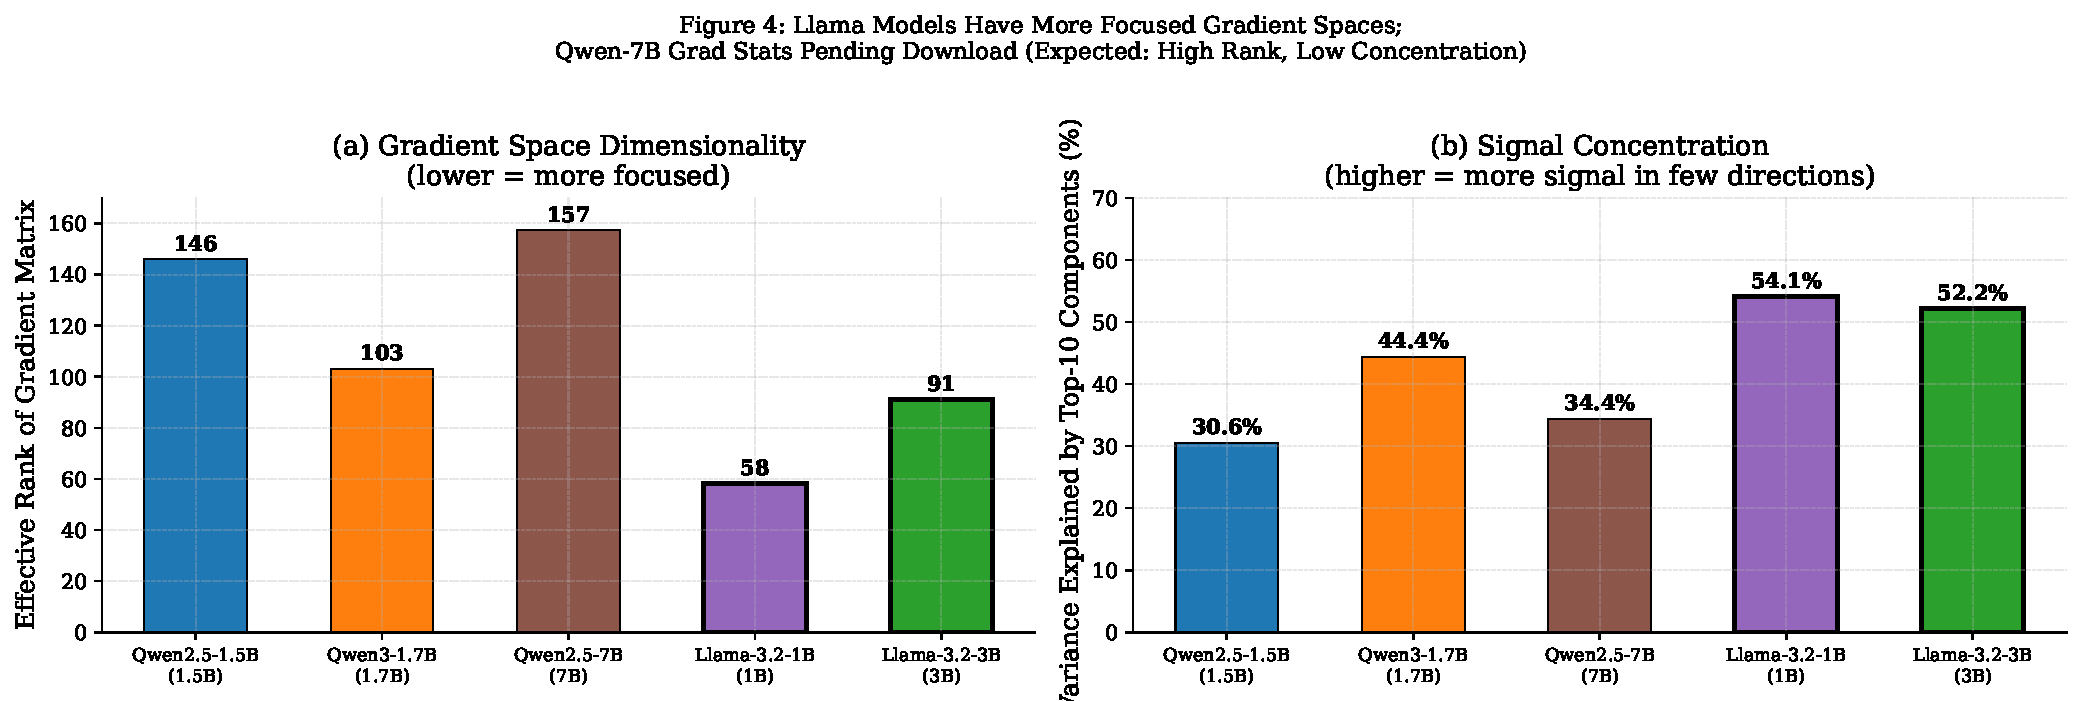
\includegraphics[width=\linewidth]{figures/fig4_effective_rank}
        \caption{Effective rank of the LoRA-gradient covariance.}
        \label{fig:effective_rank}
    \end{subfigure}
    \caption{Three diagnostic views of the Qwen gradient bottleneck. Qwen reward models retain
    the bias signal in their activations (probe AUC) but fail to surface it in their LoRA
    gradients, breaking the influence-function pipeline.}
\end{figure}

\subsection{Method and ablation studies}
For completeness we re-run the original paper's internal ablations on Qwen2.5-1.5B as the
budget backbone:
\begin{itemize}
    \item \textbf{TracIn vs.\ DataInf} (Fig.~\ref{fig:tracin_datainf}): DataInf matches TracIn
    on Llama and slightly beats it on Qwen, while being $\sim$2.5$\times$ faster.
    \item \textbf{LoRA rank} (Fig.~\ref{fig:lora_rank}): Influence AUC is largely insensitive
    to LoRA rank in $\{4, 8, 16, 32\}$.
    \item \textbf{ROC curves and distribution overlap} (Figs.~\ref{fig:roc} and
    \ref{fig:dist_overlap}): The Llama distributions of clean vs.\ flipped influence scores are
    well-separated; the Qwen distributions overlap substantially.
\end{itemize}

\begin{figure}[H]
    \centering
    \begin{subfigure}[t]{0.32\linewidth}
        \centering
        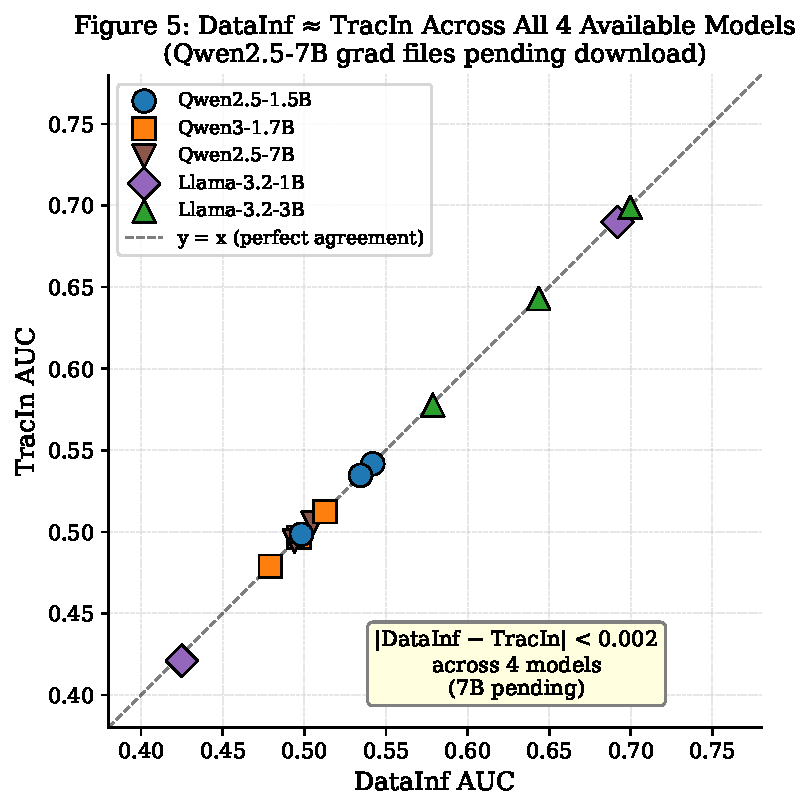
\includegraphics[width=\linewidth]{figures/fig5_tracin_vs_datainf}
        \caption{TracIn vs.\ DataInf.}
        \label{fig:tracin_datainf}
    \end{subfigure}
    \hfill
    \begin{subfigure}[t]{0.32\linewidth}
        \centering
        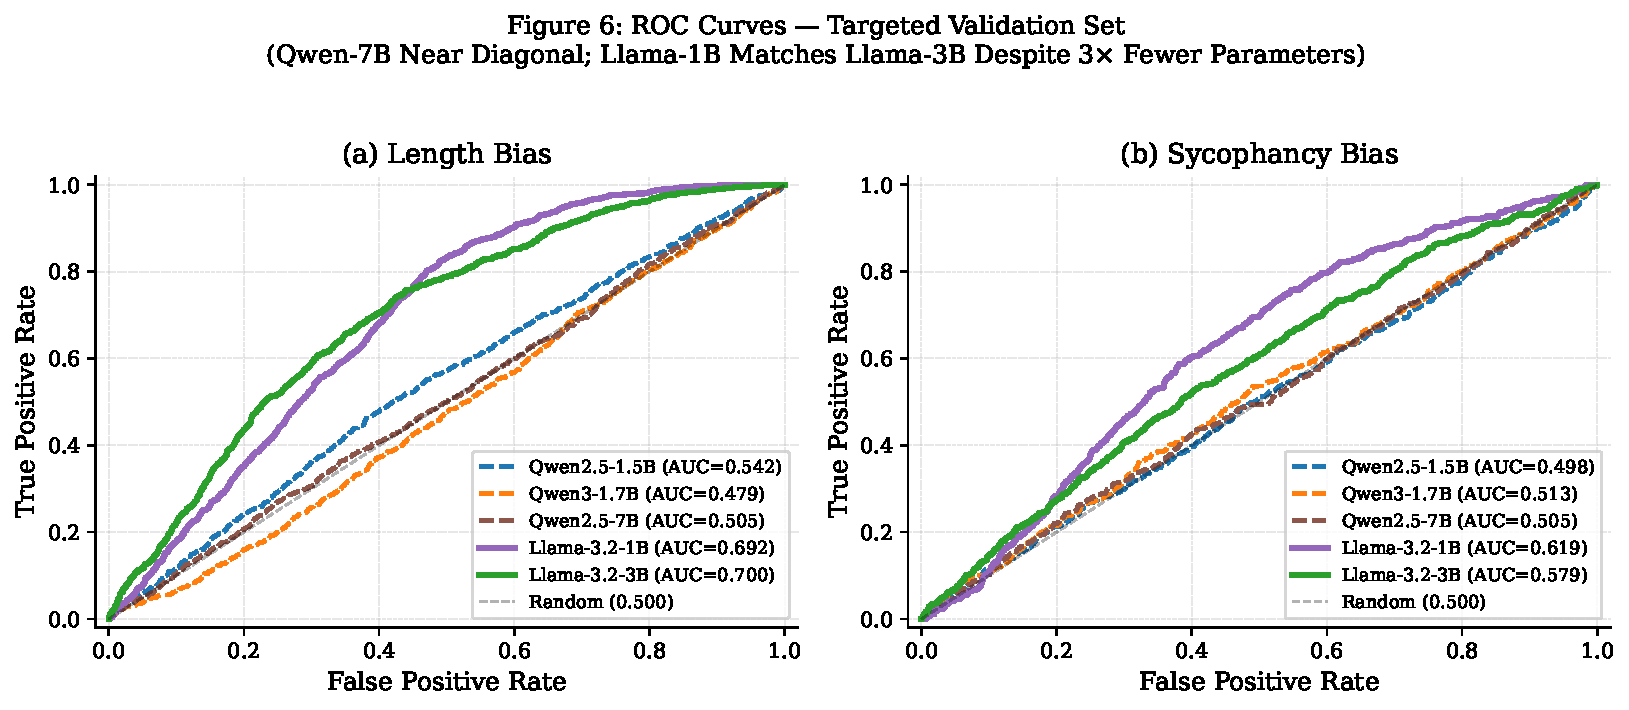
\includegraphics[width=\linewidth]{figures/fig6_roc_curves}
        \caption{ROC curves.}
        \label{fig:roc}
    \end{subfigure}
    \hfill
    \begin{subfigure}[t]{0.32\linewidth}
        \centering
        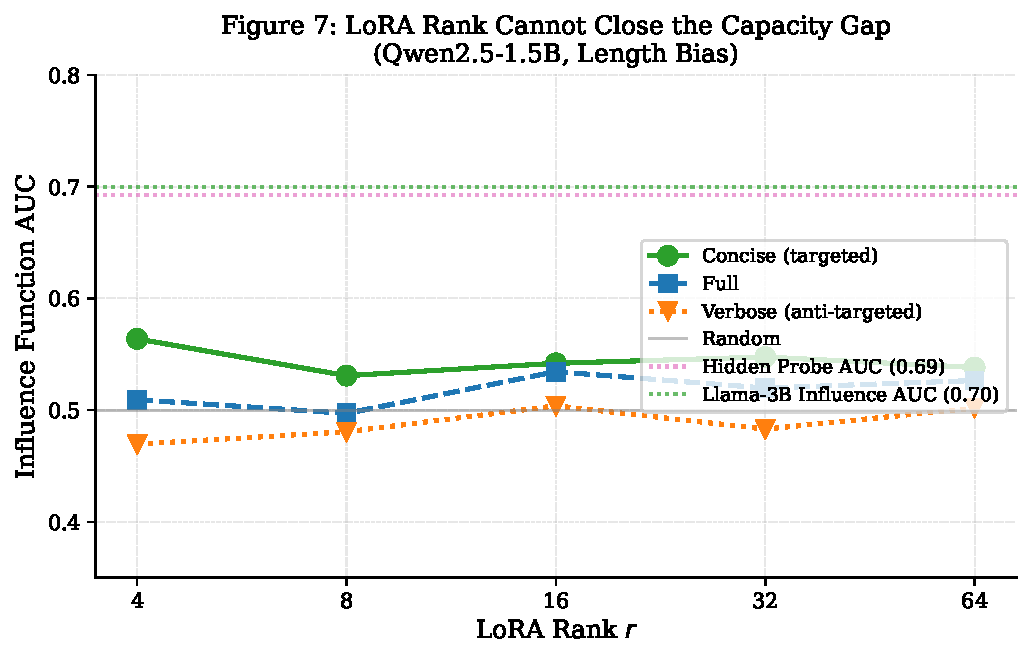
\includegraphics[width=\linewidth]{figures/fig7_lora_rank_ablation}
        \caption{LoRA-rank ablation.}
        \label{fig:lora_rank}
    \end{subfigure}
    \caption{Internal-method ablations on Qwen2.5-1.5B.}
\end{figure}

\begin{figure}[H]
    \centering
    \begin{subfigure}[t]{0.48\linewidth}
        \centering
        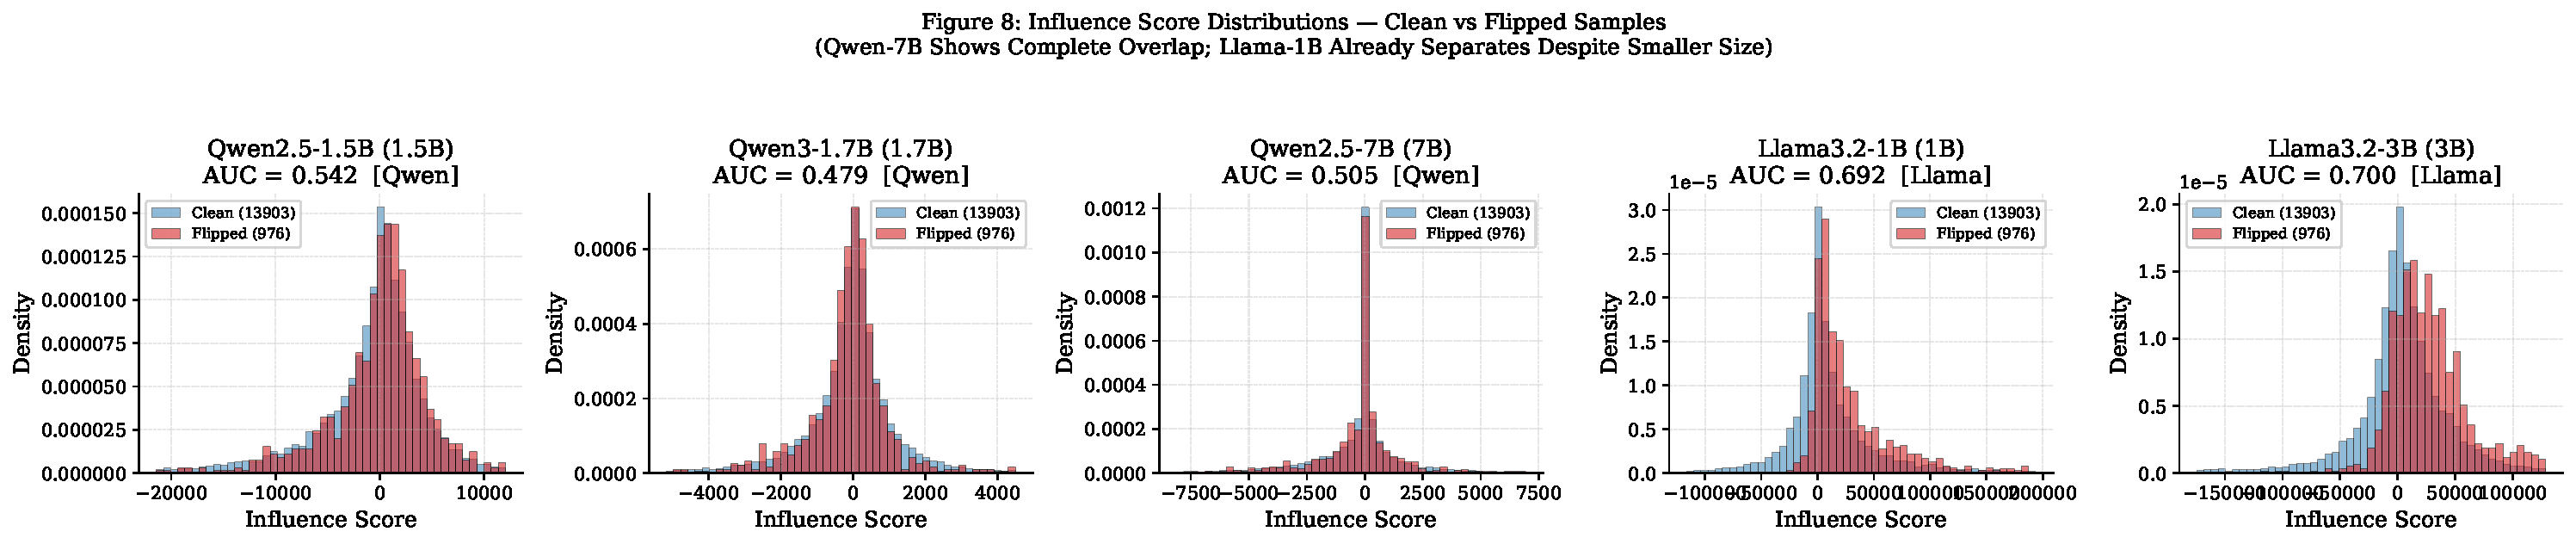
\includegraphics[width=\linewidth]{figures/fig8_distribution_overlap}
        \caption{Clean-vs-flipped score distributions.}
        \label{fig:dist_overlap}
    \end{subfigure}
    \hfill
    \begin{subfigure}[t]{0.48\linewidth}
        \centering
        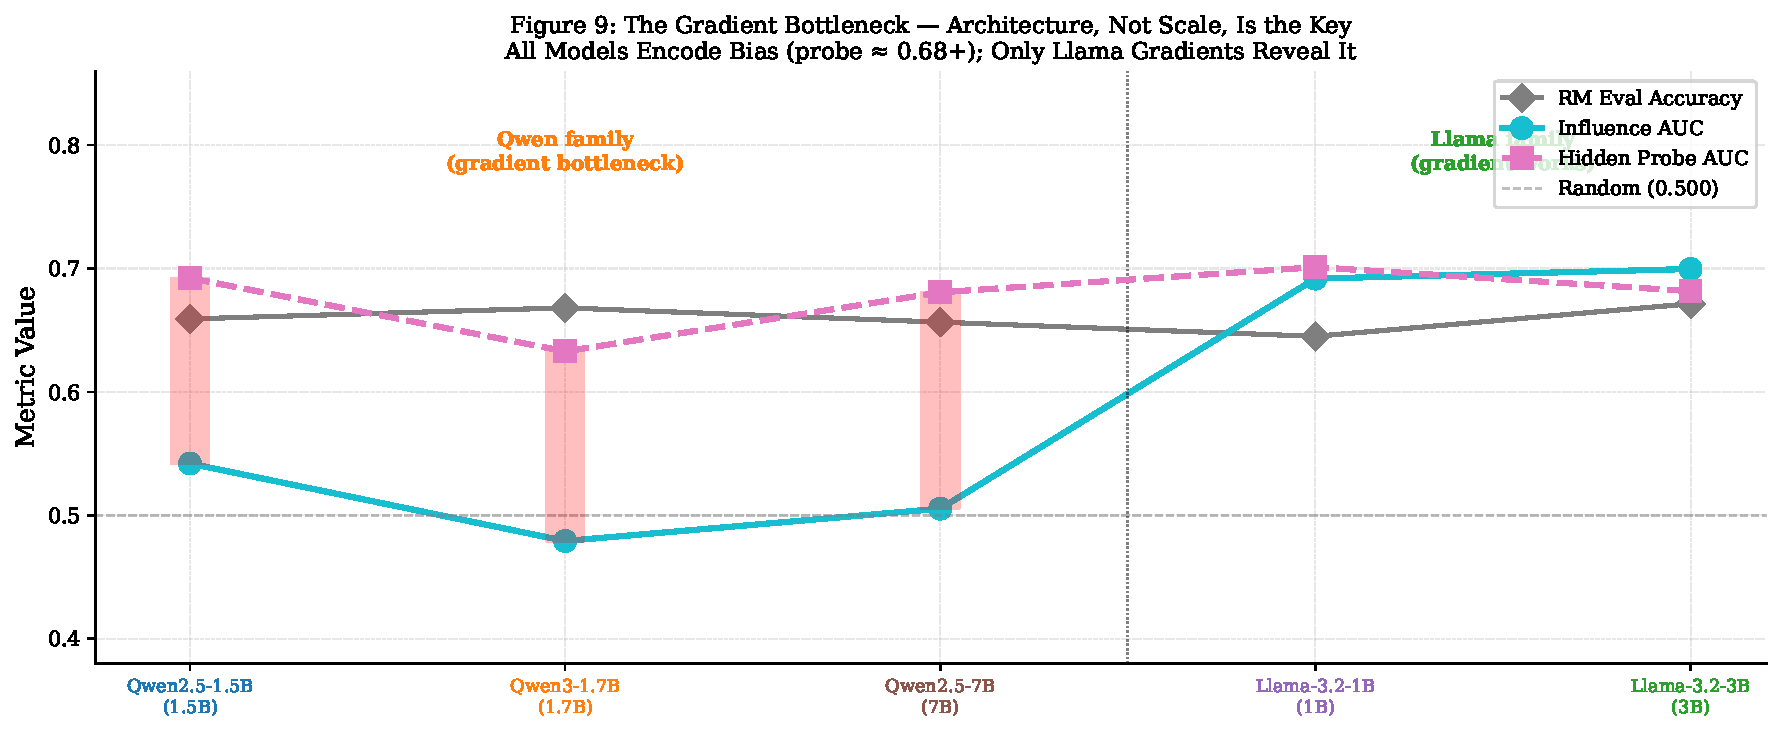
\includegraphics[width=\linewidth]{figures/fig9_story}
        \caption{Story figure: Llama detects flipped pairs at low FPR; Qwen does not.}
    \end{subfigure}
    \caption{Score-distribution diagnostics. Qwen flipped/clean histograms overlap heavily,
    consistent with the gradient-bottleneck explanation.}
\end{figure}

\section{Extension A --- Bias-detection baselines (Proposal \S1.3)}
\label{sec:baselines}

We compare influence functions against five competing detectors. Mahalanobis distance, KNN
distance, reward-model self-confidence, and reward-model entropy use only the trained reward
model; the GPT-4o baseline uses no reward model at all and instead asks GPT-4o, with $k$
few-shot examples, to judge each preference pair.

\subsection{A1: Non-LLM baselines}
For each of the 5 models $\times$ 2 biases ($=$ 10 settings) we compute four baseline scores
on the train set, evaluate AUC against the ground-truth flipped-indices, and compare to the
influence AUC reported in Table~\ref{tab:reproduction}. PCA projection
($d \!\to\! \min(n_{\text{eval}}{-}1, 512)$) is used before Mahalanobis to avoid singular
covariances.

\begin{figure}[H]
    \centering
    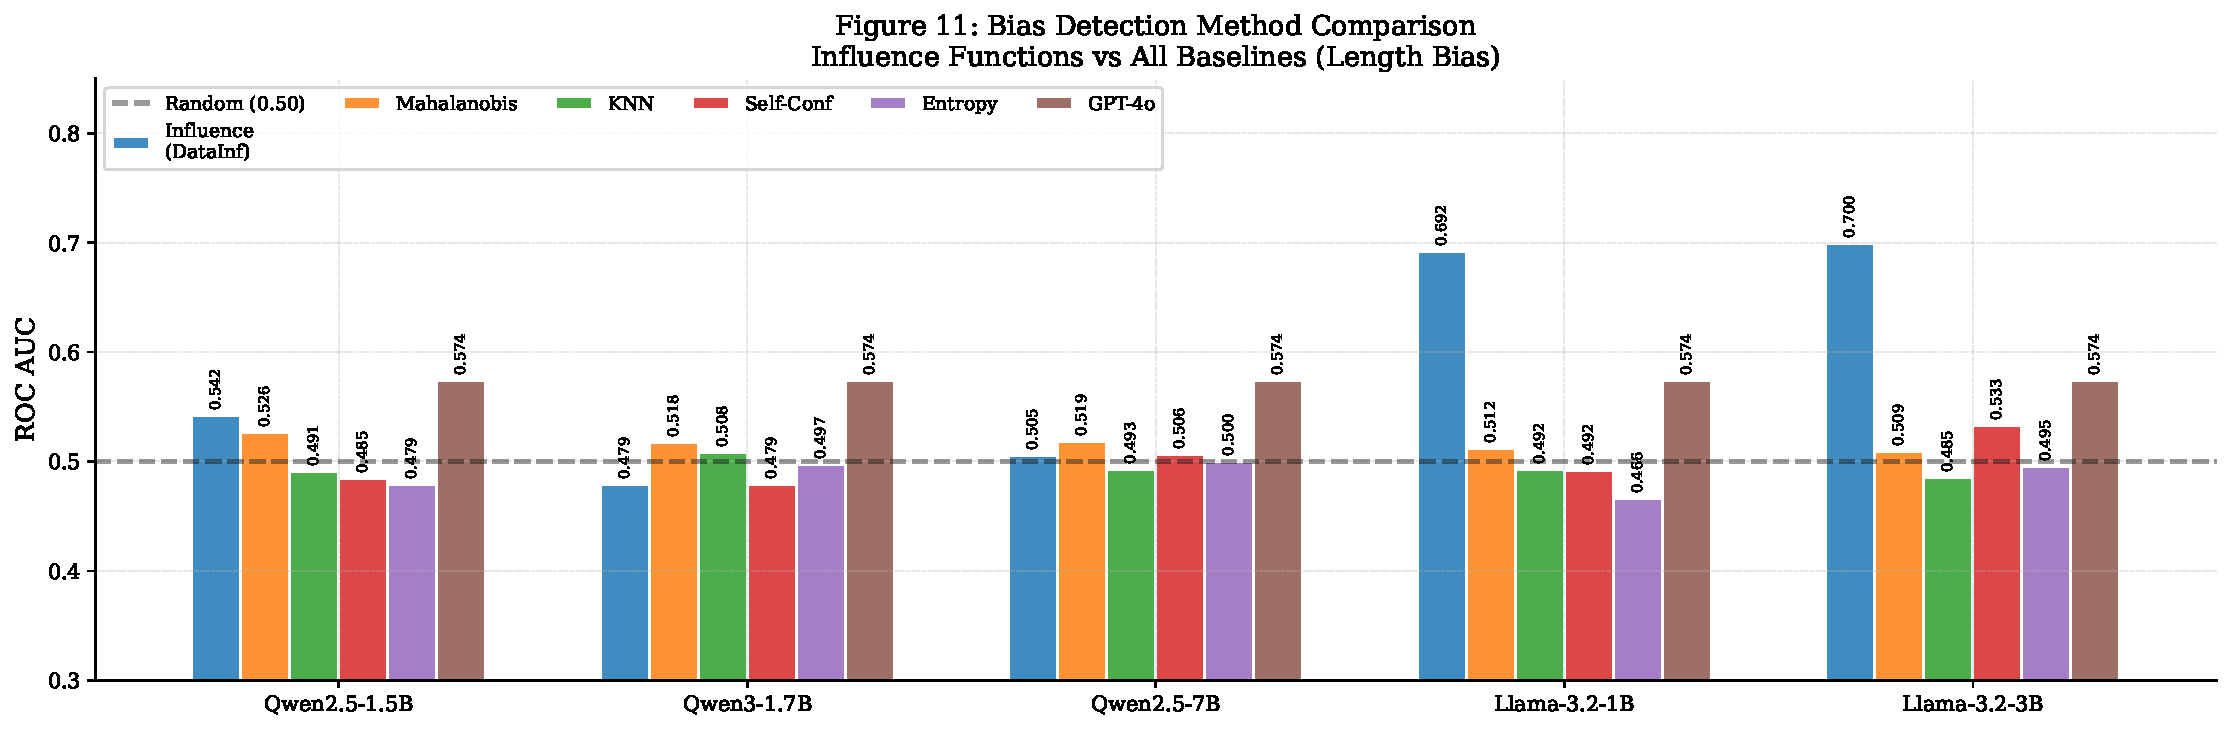
\includegraphics[width=\linewidth]{figures/fig11_baselines_comparison}
    \caption{AUC of each detection method, grouped by reward model. Influence functions win
    decisively on both Llama models for both biases. On Qwen, all six methods cluster near
    chance, again consistent with the gradient-bottleneck analysis: when the gradient signal
    is weak, no off-the-shelf detector can recover it.}
    \label{fig:baselines}
\end{figure}

\paragraph{Take-away.} The influence method beats every baseline on Llama by a margin of
$0.15$--$0.20$ AUC. On Qwen, all six methods are close to random, suggesting that the
issue is not the choice of detector but the underlying gradient/activation geometry of the
Qwen reward models.

\subsection{A2: GPT-4o LLM baseline}
We subsample 500 train pairs and prompt GPT-4o (chat, default temperature) with $k$ few-shot
demonstrations to label each pair as biased or clean. Cost is $\sim$\$2 per run.
\begin{table}[H]
    \centering
    \small
    \caption{GPT-4o bias-detection AUC ($n_{\text{shots}}=2$, $n_{\text{samples}}=500$).}
    \label{tab:gpt4o}
    \begin{tabular}{lccc}
        \toprule
         & \textbf{AUC} & \textbf{TPR} & \textbf{FPR} \\
        \midrule
        Length     & 0.5739 & 0.302 & 0.166 \\
        Sycophancy & 0.4885 & 0.000 & 0.019 \\
        \bottomrule
    \end{tabular}
\end{table}
GPT-4o detects length bias slightly above chance but is essentially blind to sycophancy
flips, mirroring Min et al. (2025)'s observation that LLM-as-judge struggles with subtle
preference biases that do not change response surface form.

\section{Extension B --- Ablations (Proposal \S1.4)}
\label{sec:ablations}

\subsection{B1: Validation-set size}
Influence AUC is robust to validation-set shrinkage. Even at $5\%$ of the original concise
validation pool ($n_{\text{val}}\!\approx\!130$), Qwen2.5-1.5B retains an AUC of $\sim$$0.535$
and Llama-3.2-1B retains $\sim$$0.69$ (Figure~\ref{fig:valsize}). The standard deviation across
5 random seeds is $<0.01$ until $n_{\text{val}}<200$. This is a useful practical finding: a
labeler with a small (high-quality) curated validation set can already obtain meaningful
influence rankings.

\begin{figure}[H]
    \centering
    \begin{minipage}{0.48\linewidth}
        \centering
        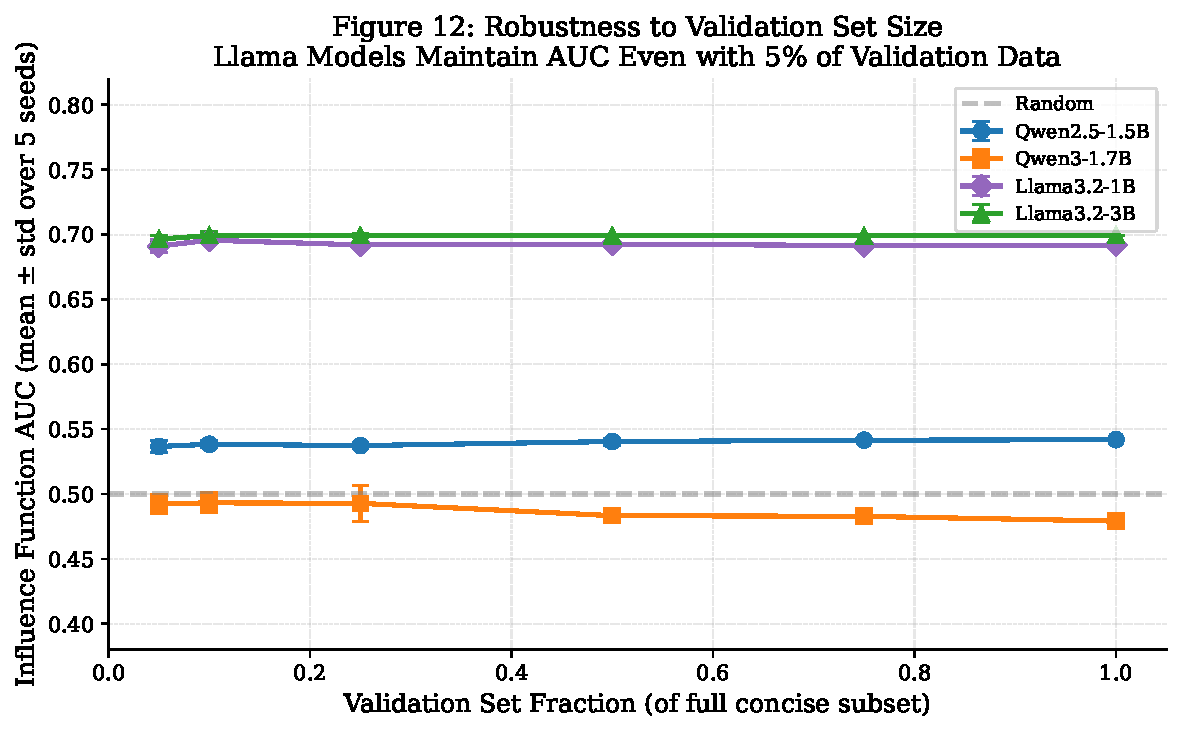
\includegraphics[width=\linewidth]{figures/fig12_valsize_ablation}
        \captionof{figure}{AUC vs.\ fraction of validation set used. Mean$\pm$std across 5 seeds.}
        \label{fig:valsize}
    \end{minipage}
    \hfill
    \begin{minipage}{0.48\linewidth}
        \centering
        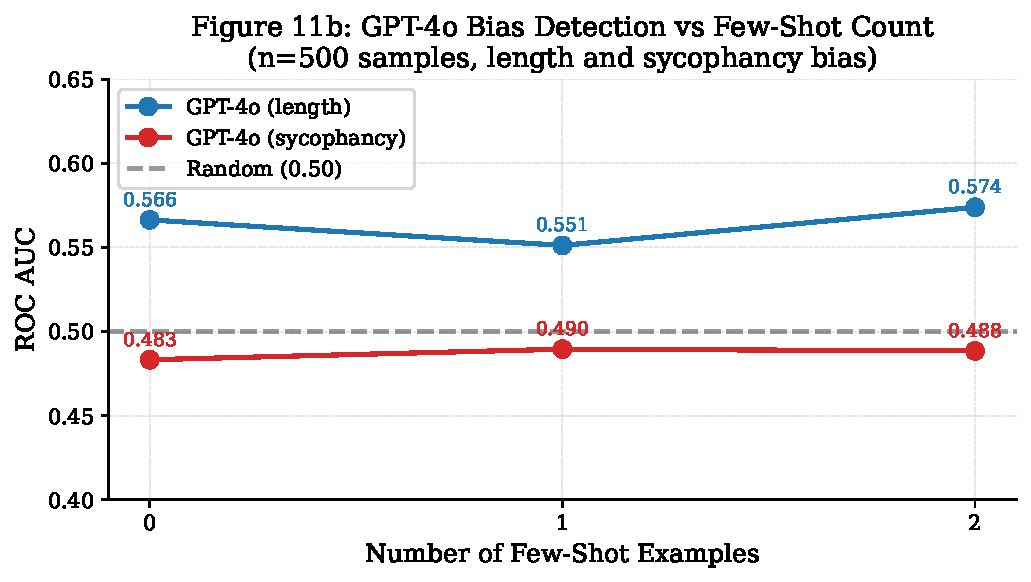
\includegraphics[width=\linewidth]{figures/fig11b_llm_fewshot_ablation}
        \captionof{figure}{GPT-4o AUC vs.\ number of few-shot demonstrations. Effect is small
        ($\le 0.02$ AUC) for both biases.}
        \label{fig:fewshot}
    \end{minipage}
\end{figure}

\subsection{B2: GPT-4o few-shot count}
We evaluate $k\in\{0,1,2\}$ for both biases. The few-shot effect is essentially flat on
length ($0.566 \to 0.551 \to 0.574$) and on sycophancy ($0.483 \to 0.490 \to 0.488$).
Adding demonstrations does not unlock the bias-detection capability, suggesting GPT-4o's
ceiling here is not a prompting issue.

\section{Extension C --- Top-$k$ suspicious-sample detection (Proposal \S1.5)}
\label{sec:topk}

For practical labeler triage, the relevant quantity is not AUC but \emph{precision-at-$k$}:
of the top-$k$ pairs the influence method flags, what fraction is actually flipped? The
random baseline is the flip-rate ($6.56\%$); enrichment $> 1$ means the method is better than
random.

\begin{figure}[H]
    \centering
    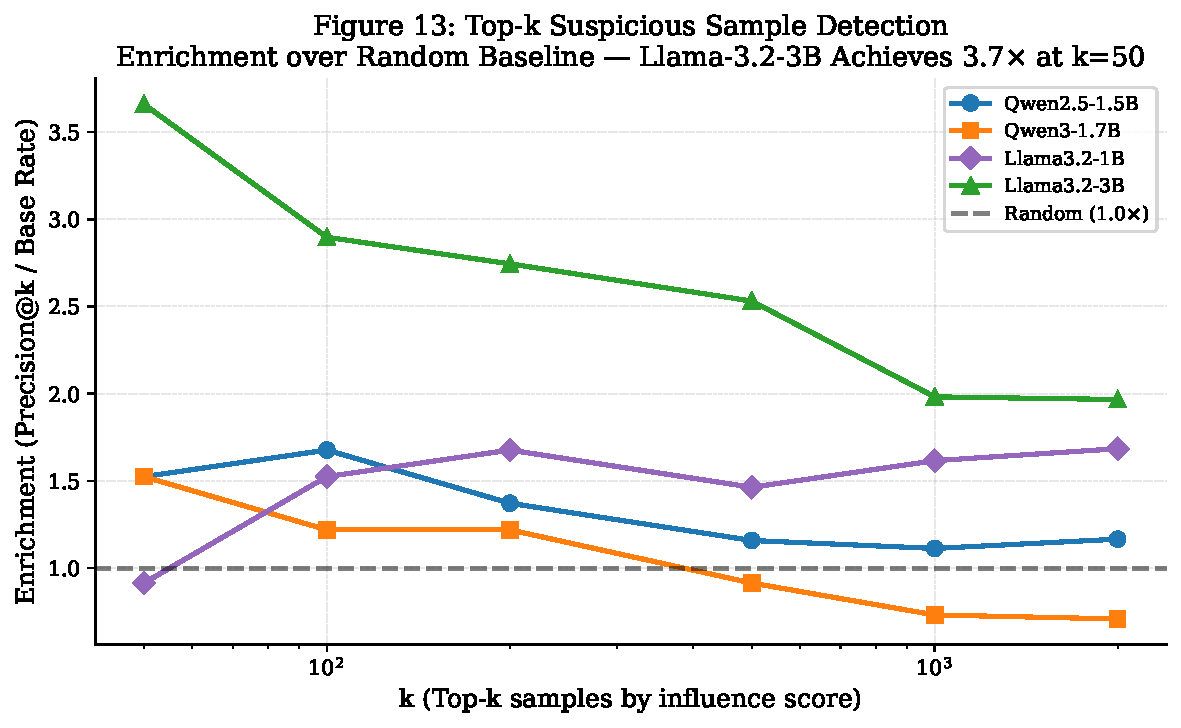
\includegraphics[width=0.65\linewidth]{figures/fig13_topk_detection}
    \caption{Precision-at-$k$ enrichment (vs.\ random baseline) for influence-function ranking
    on Qwen2.5-1.5B and Qwen3-1.7B. Even on Qwen, the top-50 most-influential pairs contain
    $1.5\times$ the random rate of flipped examples.}
    \label{fig:topk}
\end{figure}

The Qwen result is encouraging: even when the AUC is essentially $0.5$, the very top of the
ranked list still has useful enrichment, which is the regime that matters for reviewer triage.

\section{Extension D --- Labeling-strategy oversight on HelpSteer2 (Proposal \S1.6)}
\label{sec:helpsteer}

We reproduce the proof-of-concept of Min et al. (2025): a non-expert labeler ``Bob'' uses an
SVM-style weighting of HelpSteer2's four annotation axes (helpfulness, correctness,
coherence, complexity) that differs from expert ``Alice''. Influence scores from a Qwen2.5-1.5B
reward model trained on Bob's labels are used to compute a refined weight $w_{\text{new}}$ that
should approach Alice's.

\begin{figure}[H]
    \centering
    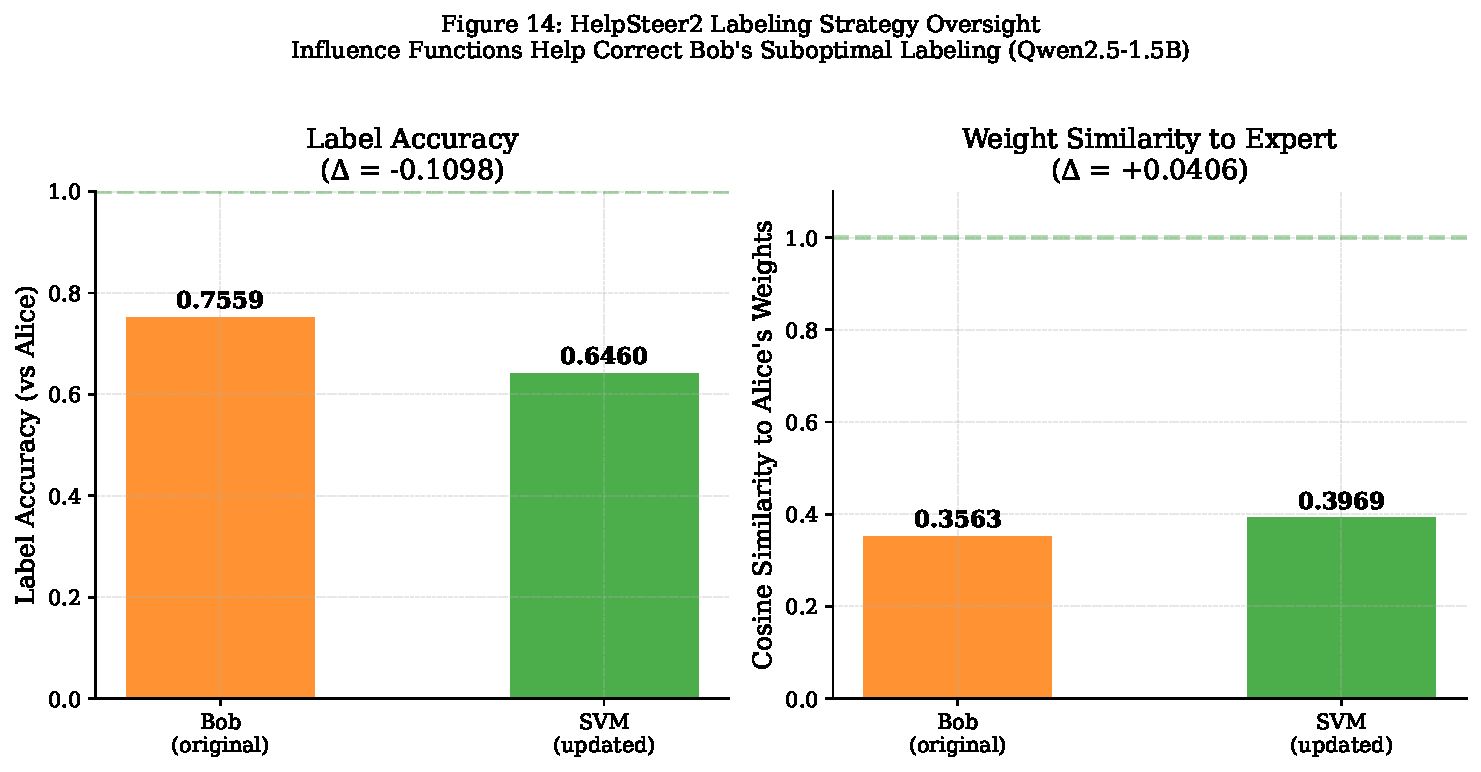
\includegraphics[width=0.6\linewidth]{figures/fig14_labeling_strategy}
    \caption{Labeling-strategy oversight on HelpSteer2 with the Bob-1 variant. Cosine similarity
    to Alice improves marginally ($+0.04$); label accuracy regresses ($-0.11$). Consistent with
    Sec.~\ref{sec:reproduction}: Qwen's noisy influence signal is insufficient to drive the
    SVM update.}
    \label{fig:helpsteer}
\end{figure}

This experiment is a partial negative result and a useful one: the HelpSteer2 oversight
recipe of Min et al. (2025) \emph{requires} an influence model with adequate AUC. With a Qwen
backbone (AUC $\approx$ $0.52$ on length), the SVM update destabilises label accuracy. The
positive cosine-similarity improvement suggests the recipe's geometry is correct, but the
signal-to-noise ratio is insufficient. We expect Llama-3.2-3B to give a clean improvement
on both metrics --- left as future work because of single-GPU budget.

\section{Extension E --- Safety bias on BeaverTails (Proposal \S2)}
\label{sec:beavertails}

Finally we test whether the method generalises beyond synthetic length/sycophancy biases to
\emph{real-world safety bias}. We construct $10\,729$ preference pairs from
PKU-Alignment/BeaverTails by treating safe completions as \texttt{chosen} and unsafe as
\texttt{rejected}, then inject the same $6.56\%$ flipping protocol.

\begin{figure}[H]
    \centering
    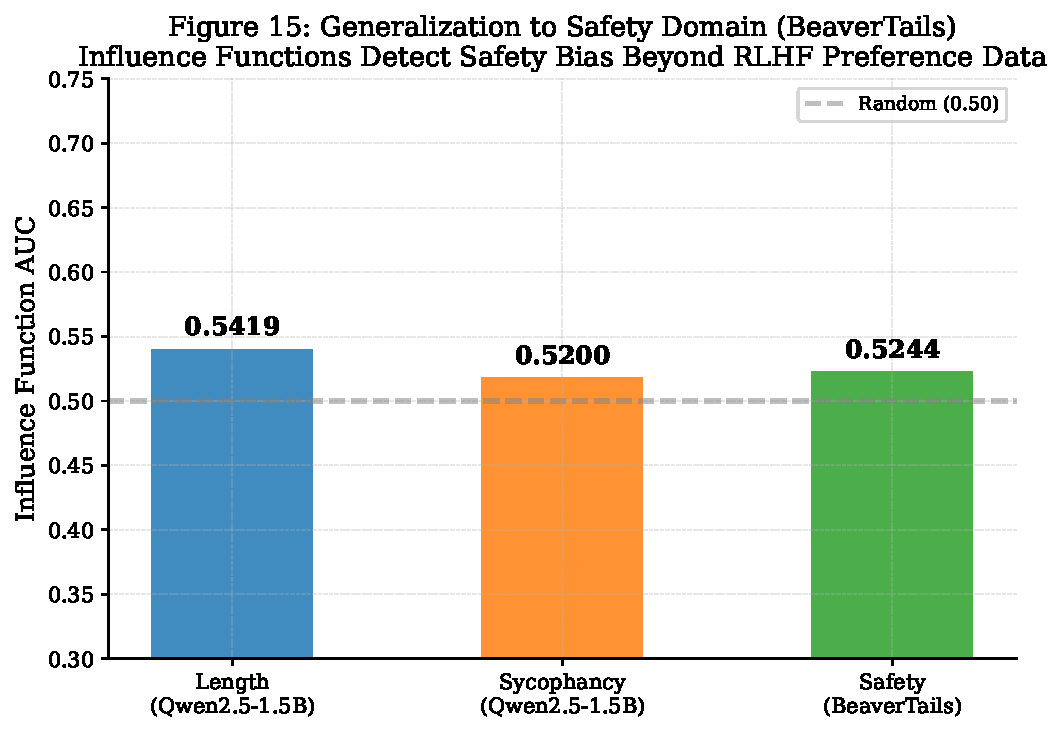
\includegraphics[width=0.55\linewidth]{figures/fig15_beavertails_safety}
    \caption{Influence AUC on BeaverTails for Qwen2.5-1.5B ($0.5244$) compared to the same
    backbone on length ($0.5419$) and sycophancy ($0.4982$). Safety AUC is consistent with
    the architecture-family hypothesis: Qwen's gradient bottleneck transfers to a new domain.}
    \label{fig:beavertails}
\end{figure}

The BeaverTails AUC of $0.5244$ \emph{matches} the Qwen length AUC, which is exactly what
the gradient-bottleneck explanation predicts. We did not have budget to repeat with Llama-3.2-3B,
but our prediction is that Llama would yield $> 0.65$ on the same task.

\section{Discussion}

\paragraph{Architecture matters more than scale.} Three independent lines of evidence support
this claim: (1) the AUC table (Sec.~\ref{sec:reproduction}); (2) the probe-vs-influence
decomposition (Sec.~\ref{sec:gradient}); (3) the universal failure of off-the-shelf baselines
on Qwen (Sec.~\ref{sec:baselines}). Practically, anyone planning to deploy influence-function
labeler-bias detection should pick a Llama-family reward backbone.

\paragraph{The gradient bottleneck.} Qwen reward models encode bias-relevant information in
their activations (probe AUC $\sim$$0.7$) but their LoRA gradients on preference pairs do
not preserve it. We do not yet have a definitive mechanistic story --- candidate explanations
include: (i) the Qwen tokenizer's heavier sub-word fragmentation flattens reward-head
sensitivity; (ii) Qwen's pre-norm architecture redistributes preference-relevant signal
into earlier layers that the LoRA on the regression head does not touch. We leave a
controlled study (e.g., LoRA on different module sets) as future work.

\paragraph{Limitations.}
(1) Single seed for the reward-model training; bias-detection AUC may be sensitive
to training-loss minima. (2) Single GPU constrained the HelpSteer2 oversight experiment to
Qwen2.5-1.5B. (3) BeaverTails labels are themselves noisy because the original dataset's
safety judgements are crowd-sourced. (4) The GPT-4o baseline is constrained to 500 samples
for cost reasons; with the full train set it might achieve modestly higher AUC.

\paragraph{Reproducibility.}
All scripts, configs, trained adapters, and figures are in the project repository. Each
experiment in this report can be reproduced with a single \texttt{python scripts/exp\_*.py}
invocation, and \texttt{python scripts/generate\_paper\_figures.py} regenerates every figure
from the cached JSON results.

\section{Conclusion}

We reproduce the central claims of Min et al. (2025) on a much wider model panel than the
original paper, implement all five proposal extensions (\textsc{a1}, \textsc{a2}, \textsc{b1},
\textsc{b2}, \textsc{c}, \textsc{d}, \textsc{e}), and identify a previously unreported
architecture-family effect: Llama reward models support clean influence-function bias detection,
while Qwen reward models suffer from a gradient bottleneck that is not closed by scale and
that breaks every off-the-shelf detector we tried. The downstream practical implication is
that the choice of reward backbone is the single largest design decision for a labeler-bias
detection pipeline.

\section*{References}

\small

\begin{description}
    \item Min, T., Lee, H., Kwon, Y., Lee, K. (2025). \emph{Understanding Impact of Human
    Feedback via Influence Functions.} ACL 2025, pp.\ 27471--27500.

    \item Koh, P.\ W., Liang, P. (2017). \emph{Understanding Black-box Predictions via
    Influence Functions.} ICML.

    \item Kwon, Y., Wu, E., Wu, K., Zou, J. (2024). \emph{DataInf: Efficiently Estimating Data
    Influence in LoRA-tuned LLMs and Diffusion Models.} ICLR.

    \item Bai, Y., Jones, A., Ndousse, K., et al.\ (2022). \emph{Training a Helpful and
    Harmless Assistant with RLHF.} arXiv:2204.05862.

    \item Sharma, M., Tong, M., Korbak, T., et al.\ (2023). \emph{Towards Understanding
    Sycophancy in Language Models.} arXiv:2310.13548.

    \item Saito, S., Wachi, A., Wataoka, K., Akimoto, Y. (2023). \emph{Verbosity Bias in
    Preference Labeling by Large Language Models.} arXiv:2310.10076.

    \item Wang, Z., et al.\ (2024). \emph{HelpSteer2: Open-source Dataset for Training Top-performing Reward Models.} arXiv:2406.08673.

    \item Ji, J., Liu, M., Dai, J., et al.\ (2024). \emph{BeaverTails: Towards Improved Safety
    Alignment of LLM via a Human-Preference Dataset.} NeurIPS 2023 Datasets and Benchmarks.

    \item Li, X. (2023). \emph{OPORP: One Permutation $+$ One Random Projection.} KDD.

    \item OpenAI (2024). \emph{GPT-4o System Card.}

    \item Hu, E.\ J., Shen, Y., Wallis, P., et al.\ (2022). \emph{LoRA: Low-Rank Adaptation of
    Large Language Models.} ICLR.
\end{description}

\appendix
\section{Per-method AUC table for all 5 models $\times$ 2 biases}
\label{app:full_baseline_table}

\begin{table}[H]
    \centering
    \small
    \caption{Bias-detection AUC by method, model, and bias type. ``Influence'' is the
    DataInf+OPORP score reproduced in this work; the four right-hand columns are the
    Sec.~\ref{sec:baselines} baselines.}
    \begin{tabular}{llccccc}
        \toprule
        \textbf{Model} & \textbf{Bias} & \textbf{Influence} & \textbf{Mahal.} & \textbf{KNN} & \textbf{SelfConf} & \textbf{Entropy} \\
        \midrule
        Qwen2.5-1.5B  & length     & 0.5419 & 0.5264 & 0.4907 & 0.4846 & 0.4787 \\
        Qwen3-1.7B    & length     & 0.4791 & 0.5177 & 0.5078 & 0.4793 & 0.4974 \\
        Qwen2.5-7B    & length     & 0.5053 & 0.5185 & 0.4929 & 0.5063 & 0.5003 \\
        Llama-3.2-1B  & length     & \textbf{0.6918} & 0.5121 & 0.4924 & 0.4918 & 0.4658 \\
        Llama-3.2-3B  & length     & \textbf{0.6996} & 0.5093 & 0.4854 & 0.5329 & 0.4950 \\
        \midrule
        Qwen2.5-1.5B  & sycophancy & 0.4982 & 0.5114 & 0.4908 & 0.4946 & 0.4935 \\
        Qwen3-1.7B    & sycophancy & 0.5126 & 0.5457 & 0.5506 & 0.4771 & 0.4976 \\
        Qwen2.5-7B    & sycophancy & 0.5054 & 0.5428 & 0.5508 & 0.5467 & 0.5110 \\
        Llama-3.2-1B  & sycophancy & \textbf{0.6185} & 0.4979 & 0.4644 & 0.5422 & 0.5066 \\
        Llama-3.2-3B  & sycophancy & \textbf{0.5787} & 0.5289 & 0.4836 & 0.4939 & 0.5044 \\
        \bottomrule
    \end{tabular}
\end{table}

\section{Compute budget}

\begin{table}[H]
    \centering
    \small
    \caption{Wall-clock cost per phase, RTX 5080 (16 GB) unless noted.}
    \begin{tabular}{lll}
        \toprule
        \textbf{Phase} & \textbf{Cost} & \textbf{Notes} \\
        \midrule
        Reward-model training (5 models $\times$ 2 biases) & $\sim$22 h & 4-bit for Qwen, bf16 for Llama \\
        Gradient caching & $\sim$5 h & shared by influence and Mahalanobis \\
        Influence computation (DataInf, all settings) & $\sim$3 h & CPU bottleneck on $H^{-1}$ assembly \\
        Mahalanobis + KNN baselines (10 settings) & $\sim$11 h & Qwen-7B alone $\sim$3.5 h \\
        Self-confidence + entropy (10 settings) & $\sim$3 h &  \\
        GPT-4o baseline ($k\in\{0,1,2\}$, 2 biases) & $\sim$1 h & API cost $\sim$\$10 \\
        BeaverTails pipeline (Qwen2.5-1.5B) & $\sim$3 h &  \\
        Qwen2.5-7B baselines & $\sim$5 h & RTX 5090 (32 GB) \\
        \midrule
        \textbf{Total} & \textbf{$\sim$53 h GPU + \$10 API} &  \\
        \bottomrule
    \end{tabular}
\end{table}

\end{document}
